\documentclass[10pt,a4paper]{article}
\usepackage[utf8]{inputenc}

\usepackage[landscape,margin=1cm]{geometry}
\usepackage[english]{babel}

\date{} % disables the default date
\title{How to Get your First Job in \textbf{Data Analytics}}
\author{Igor Shkokov}
\usepackage[default]{raleway}
\usepackage{fontawesome}
\usepackage[T1]{fontenc}

\usepackage{minted}  
\usemintedstyle{default}  

\usepackage{hyperref}
\usepackage{enumitem}
\usepackage{lipsum}

\usepackage{xcolor}
\definecolor{customcolor}{HTML}{616AC5}
\definecolor{alert}{HTML}{CD5C5C}
\definecolor{w3schools}{HTML}{4CAF50}
\definecolor{subbox}{gray}{0.60}
\definecolor{codecolor}{HTML}{FFC300}
\colorlet{xx}{customcolor}


%--------------------------Editor mode.

\usepackage
[citestyle=authoryear,
sorting=nty,	  		%Sorts bibliography by year, name, title
autocite=footnote, 		%Autocite command generates footnotes
autolang=hyphen, 		
mincrossrefs=1, 	
backend=biber]
{biblatex}

\DeclareFieldFormat{postnote}{#1}
\DeclareFieldFormat{multipostnote}{#1}
\DeclareAutoCiteCommand{footnote}[f]{\footcite}{\footcites}

\bibliography{literature}
%----------------------------------------
%--------------------------------------------------------------------------------
\usepackage{tcolorbox}

\tcbuselibrary{most,listingsutf8,minted}

\tcbset{tcbox width=auto,left=1mm,top=1mm,bottom=1mm,
right=1mm,boxsep=1mm,middle=1pt}

\newenvironment{mycolorbox}[2]{%
\begin{tcolorbox}[grow to left by=-1em,grow to right by=-1em,capture=minipage,fonttitle=\large\bfseries, enhanced jigsaw,boxsep=1mm,colback=#1!30!white,on line,tcbox width=auto, toptitle=0mm,colframe=#1,opacityback=0.7,nobeforeafter,title=#2]%
}{\end{tcolorbox}\\[0.2em]}

\newenvironment{subbox}[2]{%
\begin{tcolorbox}[capture=minipage,fonttitle=\normalsize\bfseries, enhanced jigsaw,boxsep=1mm,colback=#1!30!white,on line,tcbox width=auto,left=0.3em,top=1mm, toptitle=0mm,colframe=#1,opacityback=0.7,nobeforeafter,title=#2]\footnotesize %
}{\normalsize\end{tcolorbox}\vspace{0.1em}}

\newenvironment{multibox}[1]{%
\begin{tcbraster}[raster columns=#1,raster equal height,nobeforeafter,raster column skip=1em,raster left skip=1em,raster right skip=1em]}{\end{tcbraster}}

\newenvironment{textbox}[1]{\begin{mycolorbox}{customcolor}{#1}}{\end{mycolorbox}}

%-------------------------------
\newtcblisting{codebox}[2]{colback=codecolor!5,colframe=codecolor!80!black,listing only, 
minted options={numbers=left,style=default,fontsize=\tiny,breaklines,autogobble,linenos,numbersep=3mm},
left=5mm,enhanced,
title=#2, fonttitle=\bfseries,
listing engine=minted,minted language=#1}

%--------------------------------------------------------------------------------
\newcommand{\punkti}{~\lbrack\dots\rbrack~}

\renewenvironment{quote}
               {\list{\faQuoteLeft\phantom{ }}{\rightmargin\leftmargin}%
                \item\relax\scriptsize\ignorespaces}
               {\unskip\unskip\phantom{xx}\faQuoteRight\endlist}
               

%--------------------------------------------------------------------------------
\newcommand{\bgupper}[3]{\colorbox{#1}{\color{#2}\huge\bfseries\MakeUppercase{#3}}}
\newcommand{\bg}[3]{\colorbox{#1}{\bfseries\color{#2}#3}}

\newcommand{\mycommand}[2]{{\ttfamily\detokenize{#1}}~\dotfill{}~{\footnotesize #2}\\}
\newcommand{\sep}{{\scriptsize~\faCircle{ }~}}


\newcommand{\bggreen}[1]{\medskip\bgupper{w3schools}{black}{#1}\\[0.5em]}
\newcommand{\green}[1]{\smallskip\bg{w3schools}{white}{#1}\\}
\newcommand{\red}[1]{\smallskip\bg{alert}{white}{#1}\\}

\usepackage{multicol}
\setlength{\columnsep}{30pt}

\setlength{\parindent}{0pt}
\pagestyle{empty}

\usepackage{csquotes}

\newcommand{\loremipsum}{Lorem ipsum dolor sit amet.}


\begin{document}
\small
\begin{multicols}{3}

\maketitle
\thispagestyle{empty}
\scriptsize

%-----------------------------------------------------
\begin{textbox}{Applying}
\emph{Everyone gets through this - you will do too.}
\begin{itemize}
    \item \textbf{Apply often} (10--20 roles/week)
    \item Tailor your CV for each application \textbf{(1 custom > 5 generic)}
    \item Companies use ATS. Use \textbf{keywords.} To check CV: \href{https://www.jobscan.co/}{Jobscan}
    \item Contact HR and hiring managers via Linkedin
    \item 99\% rejection rate is normal --- \textbf{always} ask for feedback
    \item Ask friends in HR to review your CV
    \item Use \href{https://www.tealhq.com/post/xyz-resume}{XYZ method} for your CV
\end{itemize}
\end{textbox}

%-----------------------------------------------------
\begin{textboxGray}{If You're Not Getting Interviews}
\textbf{Make it impossible to ignore your application} via:
\begin{itemize}
    \item Pet projects \textbf{that stand out}
    \item Referrals inside the company
    \item Domain expertise
	\begin{itemize}
    \item Don't worry about having a polished GitHub
    \item If your approach doesn’t work - change it (after 100 app
    \item placeholder
    \item placeholder
    \item placeholder
    \item placeholder
	\end{itemize}
\end{itemize}
\end{textboxGray}
%-----------------------------------------------------

\begin{textboxWhite}{}
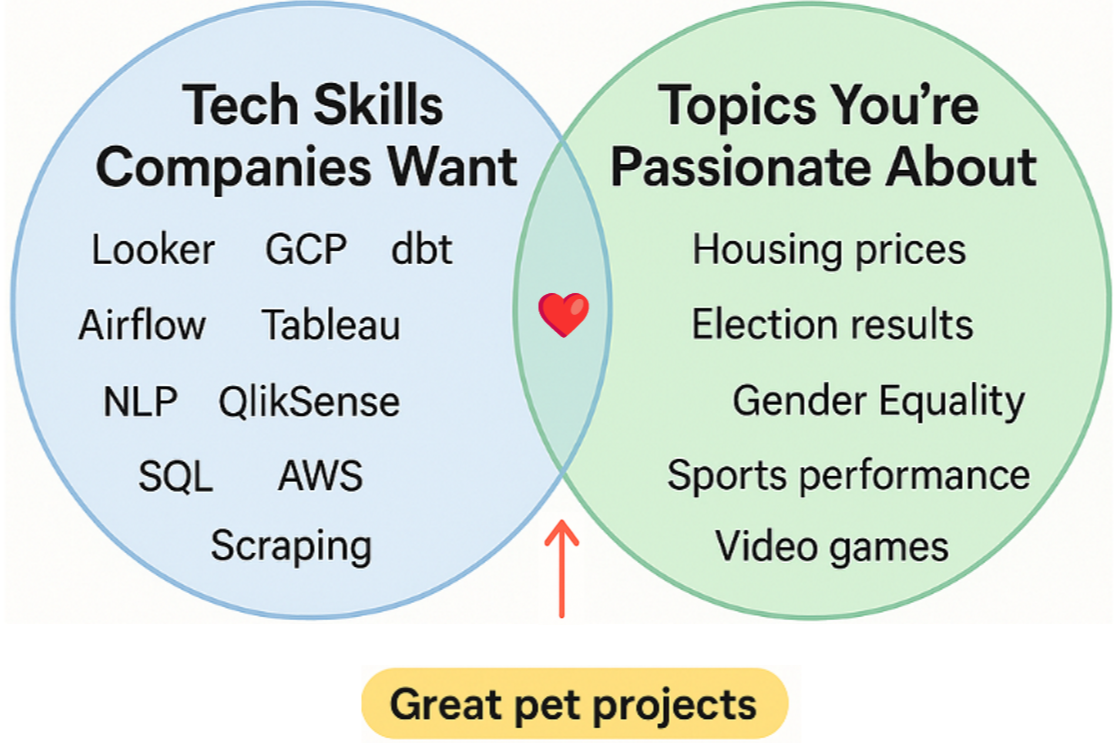
\includegraphics[width=\textwidth]{image.png}
\end{textboxWhite}

%-----------------------------------------------------
	
\begin{textboxRed}{Creating Memorable Pet Projects}
\emph{I got my first job in Data by sending \underline{\href{https://www.youtube.com/watch?v=54jvW1ulaP0&t=961s}{this video}} with every application.}

\begin{itemize}
    \item Try to find \textbf{unexpected} results
    \item Make it \textbf{showable} and \textbf{presentable} (YouTube > all)
    \item When presenting, follow the process:
	\begin{itemize}
    \item Define a Question $\Rightarrow$ Data Acquisition $\Rightarrow$ Cleaning/Wrangling $\Rightarrow$ Analysis (SQL, Python) $\Rightarrow$ Visualization (BI) $\Rightarrow$ Insights/Recommendations
	\end{itemize}

\end{itemize}

Examples:
\begin{itemize}
    \item \href{https://youtube.com/watch?v=HKuhMtrEgDE}{Paris rental prices analysis on Youtube}
    \item Another YouTube Presentation
    \item Tableau Public dashboard
    \item Medium post
    \item GitHub
    \item One-page site (GitHub Pages, Tableau)
\end{itemize}

Projects are the best for learning too.
\end{textboxRed}

%-----------------------------------------------------
\begin{textboxWhite}{}
	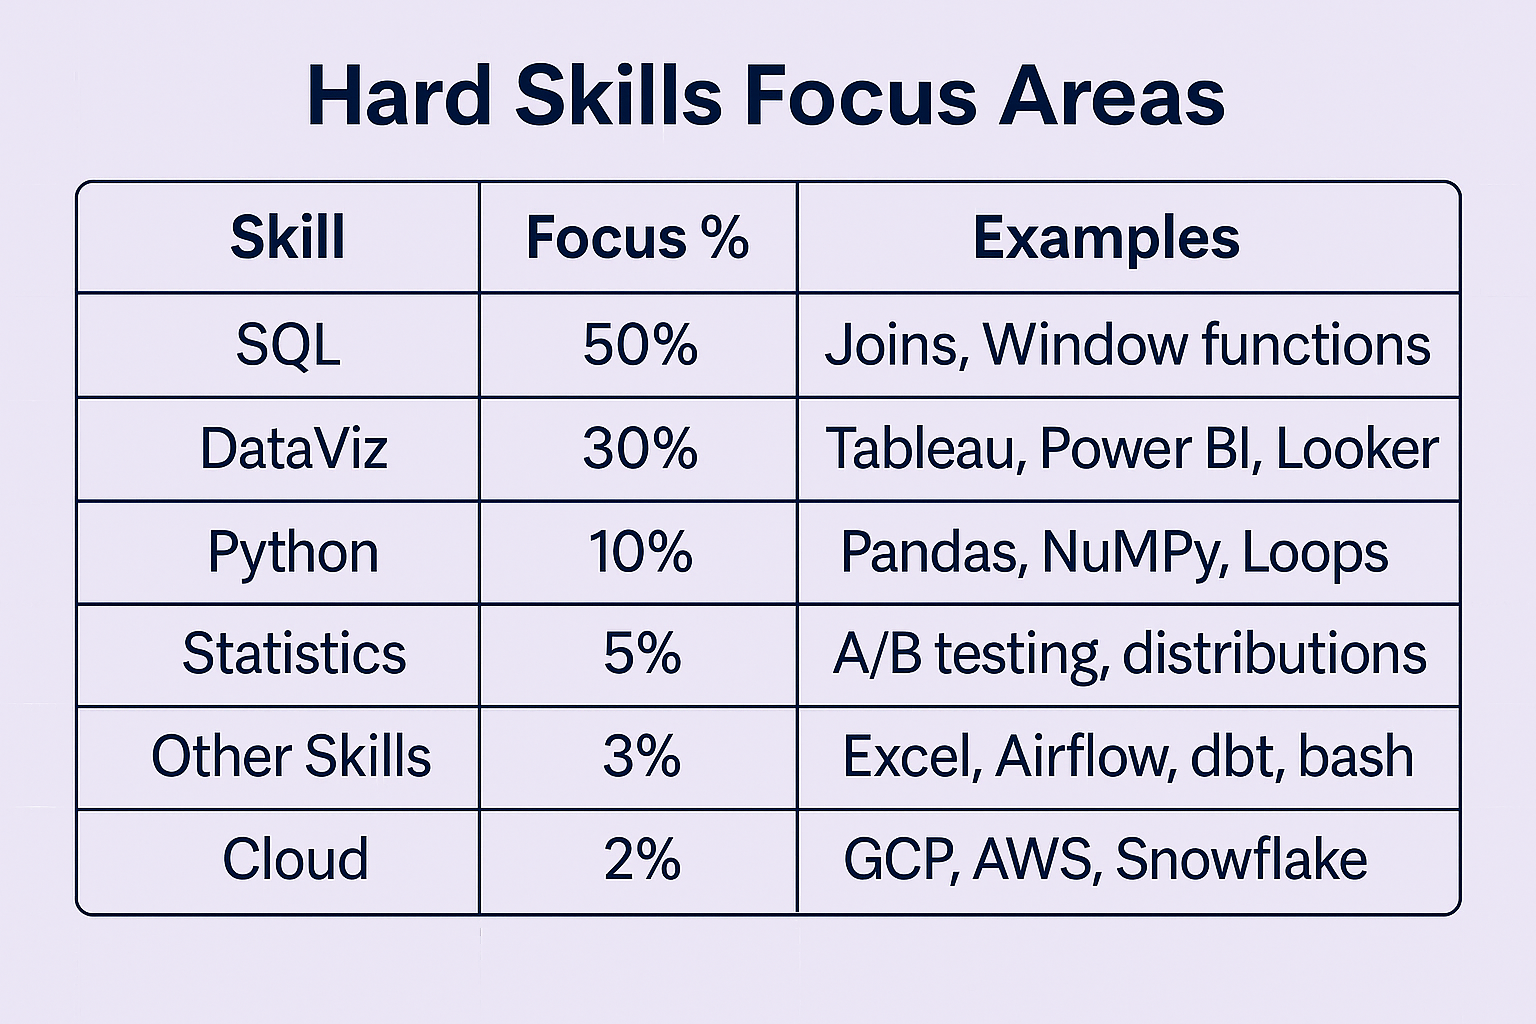
\includegraphics[width=\textwidth]{table.png}
\end{textboxWhite}

%-----------------------------------------------------
\begin{textboxGreen}{If You Get an Interview}
Well done! Here are the usual steps - some of them may be skipped or reordered, but usually:

\begin{itemize}
    \item HR call $\Rightarrow$ Technical test $\Rightarrow$ Presentation $\Rightarrow$ Another tech interview (live coding, etc) $\Rightarrow$ Team fit interview $\Rightarrow$ Offer
\end{itemize}

Each step could be the last one - there are multiple persons competing for the same position.

\begin{itemize}
    \item Recruiters often just filter --- don't expect too much
    \item If you get to a technical test, spend as much time on it as you can
    \item Smart questions are sometimes more important than smart answers - ask smart questions:
    \begin{itemize}
        \item \emph{What data challenges does your team face?}
        \item \emph{Isn't [this particular tech from their stack] outdated? Did you think about [this new tech that's more innovative]?}
    \end{itemize}
    \item On each step, ask how many other candidates do they see on this step. Even if they won't answer, you'll get an idea.
    \item Put yourself in shoes of your interviewers. What are their pains? What are they trying to optimize for?
\end{itemize}
\end{textboxGreen}

%-----------------------------------------------------
\begin{textboxYellow}{Courses and Practice}
\emph{Practice often, especially before a live coding test.}

\begin{itemize}
    \item The best: \href{https://datacamp.com/}{\textbf{DataCamp}}
    \item SQL: \href{https://datalemur.com/}{DataLemur}, \href{https://www.sqlnoir.com/}{SQL Noir}, \href{https://mystery.knightlab.com/}{SQL Mystery}
    \item Datasets: \href{https://www.kaggle.com/}{Kaggle}
    \item Coding challenges: \href{https://leetcode.com/}{Leetcode}, \href{https://www.stratascratch.com/}{Stratascratch}
\end{itemize}
\end{textboxYellow}

%-----------------------------------------------------
\begin{textboxYellow}{What to Read}
\textbf{Blogs:}
\begin{itemize}
    \item \href{https://towardsdatascience.com/}{Towards Data Science}
    \item \href{https://www.kdnuggets.com/}{Kdnuggets}
    \item \href{https://ourworldindata.org/}{Our World in Data}
    \item \href{https://www.voronoiapp.com/}{Voronoi}
    \item \href{https://reddit.com/r/dataanalysis/}{\texttt{r/dataanalysis}}
\end{itemize}
\textbf{Newsletters:} \href{https://tldr.tech/newsletters}{TLDR}, \href{https://flowingdata.com/newsletter/}{FlowingData}, \href{https://www.blef.fr/}{Blef.fr}, \href{https://www.holoniq.com/newsletters}{HolonIQ}

\textbf{Books:}
\begin{itemize}
    \item \href{https://www.amazon.com/Designing-Your-Life-Well-Lived-Joyful/dp/1101923083}{Designing Your Life} (Part 7: How Not to Get a Job)
    \item \href{https://www.amazon.com/Wishcraft-How-What-Really-Want/dp/0345465180}{Wishcraft}
\end{itemize}
\end{textboxYellow}

%-----------------------------------------------------
\begin{textbox}{One Last Thought}
\emph{What would you do this if you had unlimited money?}
\end{textbox}
%-----------------------------------------------------


\date{\today}
\end{multicols}
\end{document}
